\renewcommand{\chaptername}{BAB}
%-----------------------------------------------------------------------------%
\chapter{METODOLOGI PENELITIAN}
%-----------------------------------------------------------------------------%

\vspace{4.5pt}
\setlength{\parskip}{0.5em}
\section{Rancangan Penelitian}\label{sec:rancangan_penelitian}
Tipe Penelitian yang peneliti gunakan disini merupakan penelitian terapan langsung. Peneliti melakukan
\textit{development} secara langsung terhadap Argo CD yang akan digunakan pada sistem bare-metal (\textit{non-cloud}) yang mengembangkan fitur continous integration dengan ArgoCD

\begin{figure}[h]
    \centering
    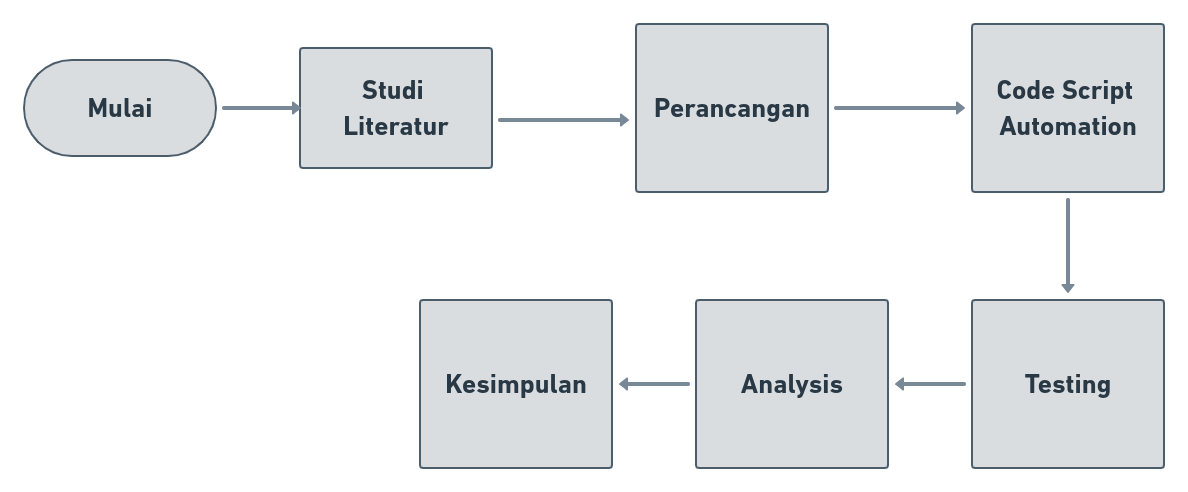
\includegraphics[width=1\textwidth]{figures/Tahapan Skripsi.png}
    \caption{Rancangan Penelitian}
\end{figure}

\section{Studi Literatur}\label{sec:studi_literatur}
Pada tahap studi literatur, peneliti mengumpulkan teori-teori,
konsep, dan temuan penelitian terdahulu yang relevan sebagai landasan dalam melakukan pengembangan dan implementasi automasi deployment menggunakan Argo CD pada lingkungan Kubernetes.
Studi literatur ini dilakukan dengan menelaah berbagai sumber seperti buku, jurnal nasional dan internasional, serta dokumentasi resmi terkait GitOps dan Argo CD.

Peneliti mempelajari konsep dasar GitOps yang menekankan penggunaan repository Git sebagai sumber kebenaran (single source of truth) untuk seluruh konfigurasi dan deployment aplikasi \cite{Weaveworks2017}.
Selain itu, peneliti juga mengkaji dokumentasi resmi Argo CD yang menjelaskan fitur, arsitektur, serta best practice dalam penerapannya pada workflow CI/CD \cite{ArgoCDDocs}.
Penelitian terdahulu dari Korhonen \cite{Korhonen2021} menjadi salah satu referensi utama, di mana dijelaskan penerapan Argo CD untuk meningkatkan konsistensi, efisiensi, dan auditability proses deployment aplikasi pada Kubernetes.

Selain itu, peneliti juga menelaah studi komparatif antara Argo CD dan tools GitOps lain seperti Flux yang dilakukan oleh Sharma et al. \cite{Sharma2022},
serta kajian terkait tantangan keamanan dalam implementasi Argo CD yang dibahas oleh Kumar \cite{Kumar2023}. Dengan mengkaji berbagai referensi tersebut,
peneliti memperoleh pemahaman yang komprehensif mengenai teori dan praktik automasi deployment berbasis GitOps, sehingga dapat merancang dan mengimplementasikan solusi yang sesuai dengan kebutuhan penelitian.

\subsection{Perancangan (Design)}
Setelah melakukan tahap studi literatur dan analisis kebutuhan sistem, tahap selanjutnya adalah melakukan perancangan sistem automasi deployment yang akan diimplementasikan. Pada tahap studi literatur yang telah dilakukan, peneliti mengambil rancangan dasar dari penelitian-penelitian terdahulu, khususnya model GitOps yang dibahas oleh Ramadoni \cite{Ramadoni2021} dan arsitektur Argo CD yang dijelaskan oleh Korhonen \cite{Korhonen2021}.

Pada tahap ini, peneliti melakukan modifikasi terhadap rancangan yang sudah ada untuk mengadaptasi implementasi Argo CD pada lingkungan bare-metal (non-cloud) dengan memanfaatkan platform virtualisasi Proxmox. Modifikasi ini penting dilakukan karena sebagian besar implementasi GitOps dan Argo CD yang ada di literatur berfokus pada lingkungan cloud \cite{Bolscher2019}, sementara penelitian ini bertujuan untuk mengimplementasikan solusi serupa pada infrastruktur on-premise.

Perancangan yang dilakukan meliputi beberapa aspek utama, yaitu:

\begin{enumerate}
    \item Perancangan arsitektur sistem automasi deployment menggunakan Argo CD pada lingkungan Kubernetes yang berjalan di atas Proxmox
    \item Perancangan alur kerja sistem sesuai dengan pendekatan pull-based deployment yang merupakan karakteristik utama dari GitOps \cite{Weaveworks2017}
    \item Perancangan mekanisme continuous integration yang terintegrasi dengan Argo CD untuk membentuk pipeline CI/CD yang lengkap
    \item Perancangan strategi deployment dan rollback yang efektif untuk aplikasi berbasis microservice
\end{enumerate}

Langkah terakhir yang akan dilakukan adalah merancang konfigurasi dan manifest Kubernetes yang diperlukan untuk implementasi Argo CD pada lingkungan bare-metal, serta menyiapkan dokumentasi teknis yang diperlukan untuk proses implementasi. Dokumentasi ini akan mencakup detail tentang arsitektur sistem, komponen-komponen utama, dan alur kerja dari proses deployment yang diusulkan.
\newpage
